\chapter{Design and Implementation}\label{implement}

    In this chapter, the implementation details will be explained in many aspects, including Java Native Interface,
    human detection and distance calculation.

    \section{MoSCoW Statement}

        \subsection{Must have}
            \begin{itemize}
                \setlength\itemsep{1em}
                \item The application \textbf{must} be able to detect people in the given image or video.
                \item The application \textbf{must} be able to determind distancing between people in the given image or video.
                \item The application \textbf{must} save the processed image of video.
                \item The application \textbf{must} allow user to choose image or video from device's storage.
            \end{itemize}

        \subsection{Should have}
            \begin{itemize}
                \item The application \textbf{should} be able to stream video from camera.
                \item The application \textbf{should} be able to show detected people on camera.
                \item The application \textbf{should} support parallel computing.
            \end{itemize}

        \subsection{Could have}
            \begin{itemize}
                \item The application \textbf{could} choose computation options between sequencial or parallelism.
                \item The application \textbf{could} support NEON techonology.
                \item The application \textbf{could} be able to process the given tasks in background.
            \end{itemize}
        \subsection{Won't have}
            \begin{itemize}
                \item The application \textbf{won't} other objects which are not human.
                \item The application \textbf{won't} support GPU computation.
            \end{itemize}

    \section{Interface Design}
        - open an app, you will face the main menu \ref{appendix-b:mainMenu}.
        - there are three buttons in the main menu: browsing video, browsing picture and opening a camera.
        - When a video or image button is clicked, the user will be navigated to file picker \ref{appendix-b:filePicker}
        - When a file is chosen, the file will be processed in the background, and the status bar will be updated regarding the progress \ref{appendix-b:statusBar}.
        - When processing is done, video or image will be shown \ref{appendix-b:result}
        - red is social distancing  violation, green is OK.
        - Or user can use camera for real-time detection
        - user will be navigated to camera activity \ref{appendix-b:camera}
        - application will process and show in real-time

    \section{Preparation}
        This application is implemented on the Android Operating System,
        and the target Software Development Kit (SDK) version is set at level 29, namely Android Q.
        This application is compiled and built by Android Studio version 3.5.3,
        and CMake is used for compiling C++ library with C++ version 11.
        Furthermore, OpenCV version 4.4.0, which is built as a shared library, is used for image processing and object detection.
        For object detection model, two models are used: You Only Look Once and MobileNet SSD.

    \section{Java Native Interface}
        Implementation is divided into 3 layers.
            The first layer is a Java layer, which mainly interacts with a user,
            checks permissions, handles activity lifecycle, communicates with Java Native Interface (JNI), and loads native libraries.
                Native libraries are compiled and built into shared libraries by a Native Development Kit (NDK).
            The second layer is JNI, which is written in C or C++.
                The task of the JNI layer is an intermediate connection between the Java layer and a C++ layer.
            The last layer is the C++ layer, which alternatively performs calculation tasks,
            including Deep Neural Network and distance calculation.

        \begin{figure}[!ht]
            \centering
            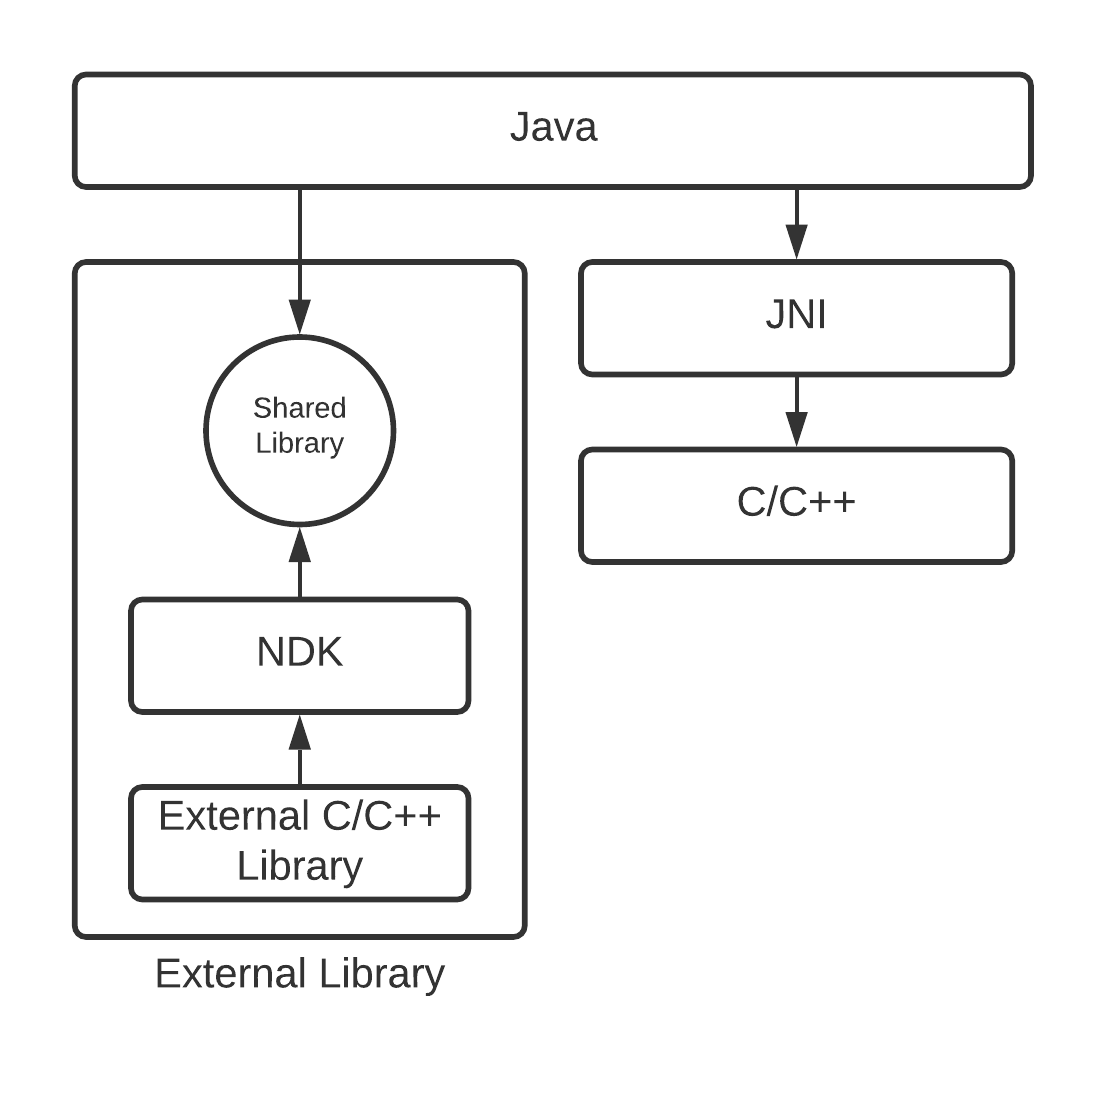
\includegraphics[width=4in]{images/chapter3/application-layers.png}
            \caption{Application Layers}
            \label{systemOverview}
        \end{figure}

        However, Deep Neural Network and distance calculation can be implemented in all layers.
        According to Android Developer Guide \cite{ANDROID-01},
        Native Development Kit (NDK) is recommended for compiling C and C++ code into the native library,
        which is able to achieve higher performance.
        Thus, executing both tasks in the JNI and C++ layer gains a better performance.
        Furthermore, there are two advantages to implementing JNI.
            The first advantage is reducing JNI calling. Performing both tasks in an application layer have to call JNI methods many times,
                and this is expensive and cost overhead.
                Thus, manually implementing JNI reduces the number of JNI calls.
            The second advantage is memory management. C++ is able to access values in the memory by using a pointer.
                Thus, values can be directly accessed without copying.

        Java and JNI communicate through native function, which is written in the Java layer.
        Memory addresses of the pre-processed frame in Mat format will be pass as a parameter through native function,
        and it will be converted from Java type to Native type.
        Then, the given addresses will be converted back into Mat format.

\begin{lstlisting}[caption={Java Native Function},captionpos=b]
    public class NativeLib {
        static {
            System.loadLibrary("native-lib");
        }

        public native static void process(long imageAddr);
    }
\end{lstlisting}

\begin{lstlisting}[caption={C++ JNI Method},captionpos=b]
    Java_com_jinkawin_dissertation_NativeLib_process(jlong matAddr){
        Mat &frame = *(Mat *) matAddr;
        ImageProcessor::process(frame);
    }
\end{lstlisting}

    \section{Social Distancing Detection}
        % Intro to detection
        There are three main processes that are implemented to determine social distancing violation from the image and video.

        The first process is pre-processing the given image, video, or video stream.
        The given video will be extracted into an array of images.
        Then, images will be converted into Bitmap and Mat format with RGBA colour model respectively.
        After that, the colour will be converted, which depends on the detection model.
        As mentioned in section 4.1, there are two detection models are used for detecting humans in the given picture and video: YOLO model and MobileNet SSD model.
        Colour will be converted to RGB if the detection model is YOLO,
        while MobileNet SSD requires BGR colour model.

        \begin{figure}[!ht]
            \centering
            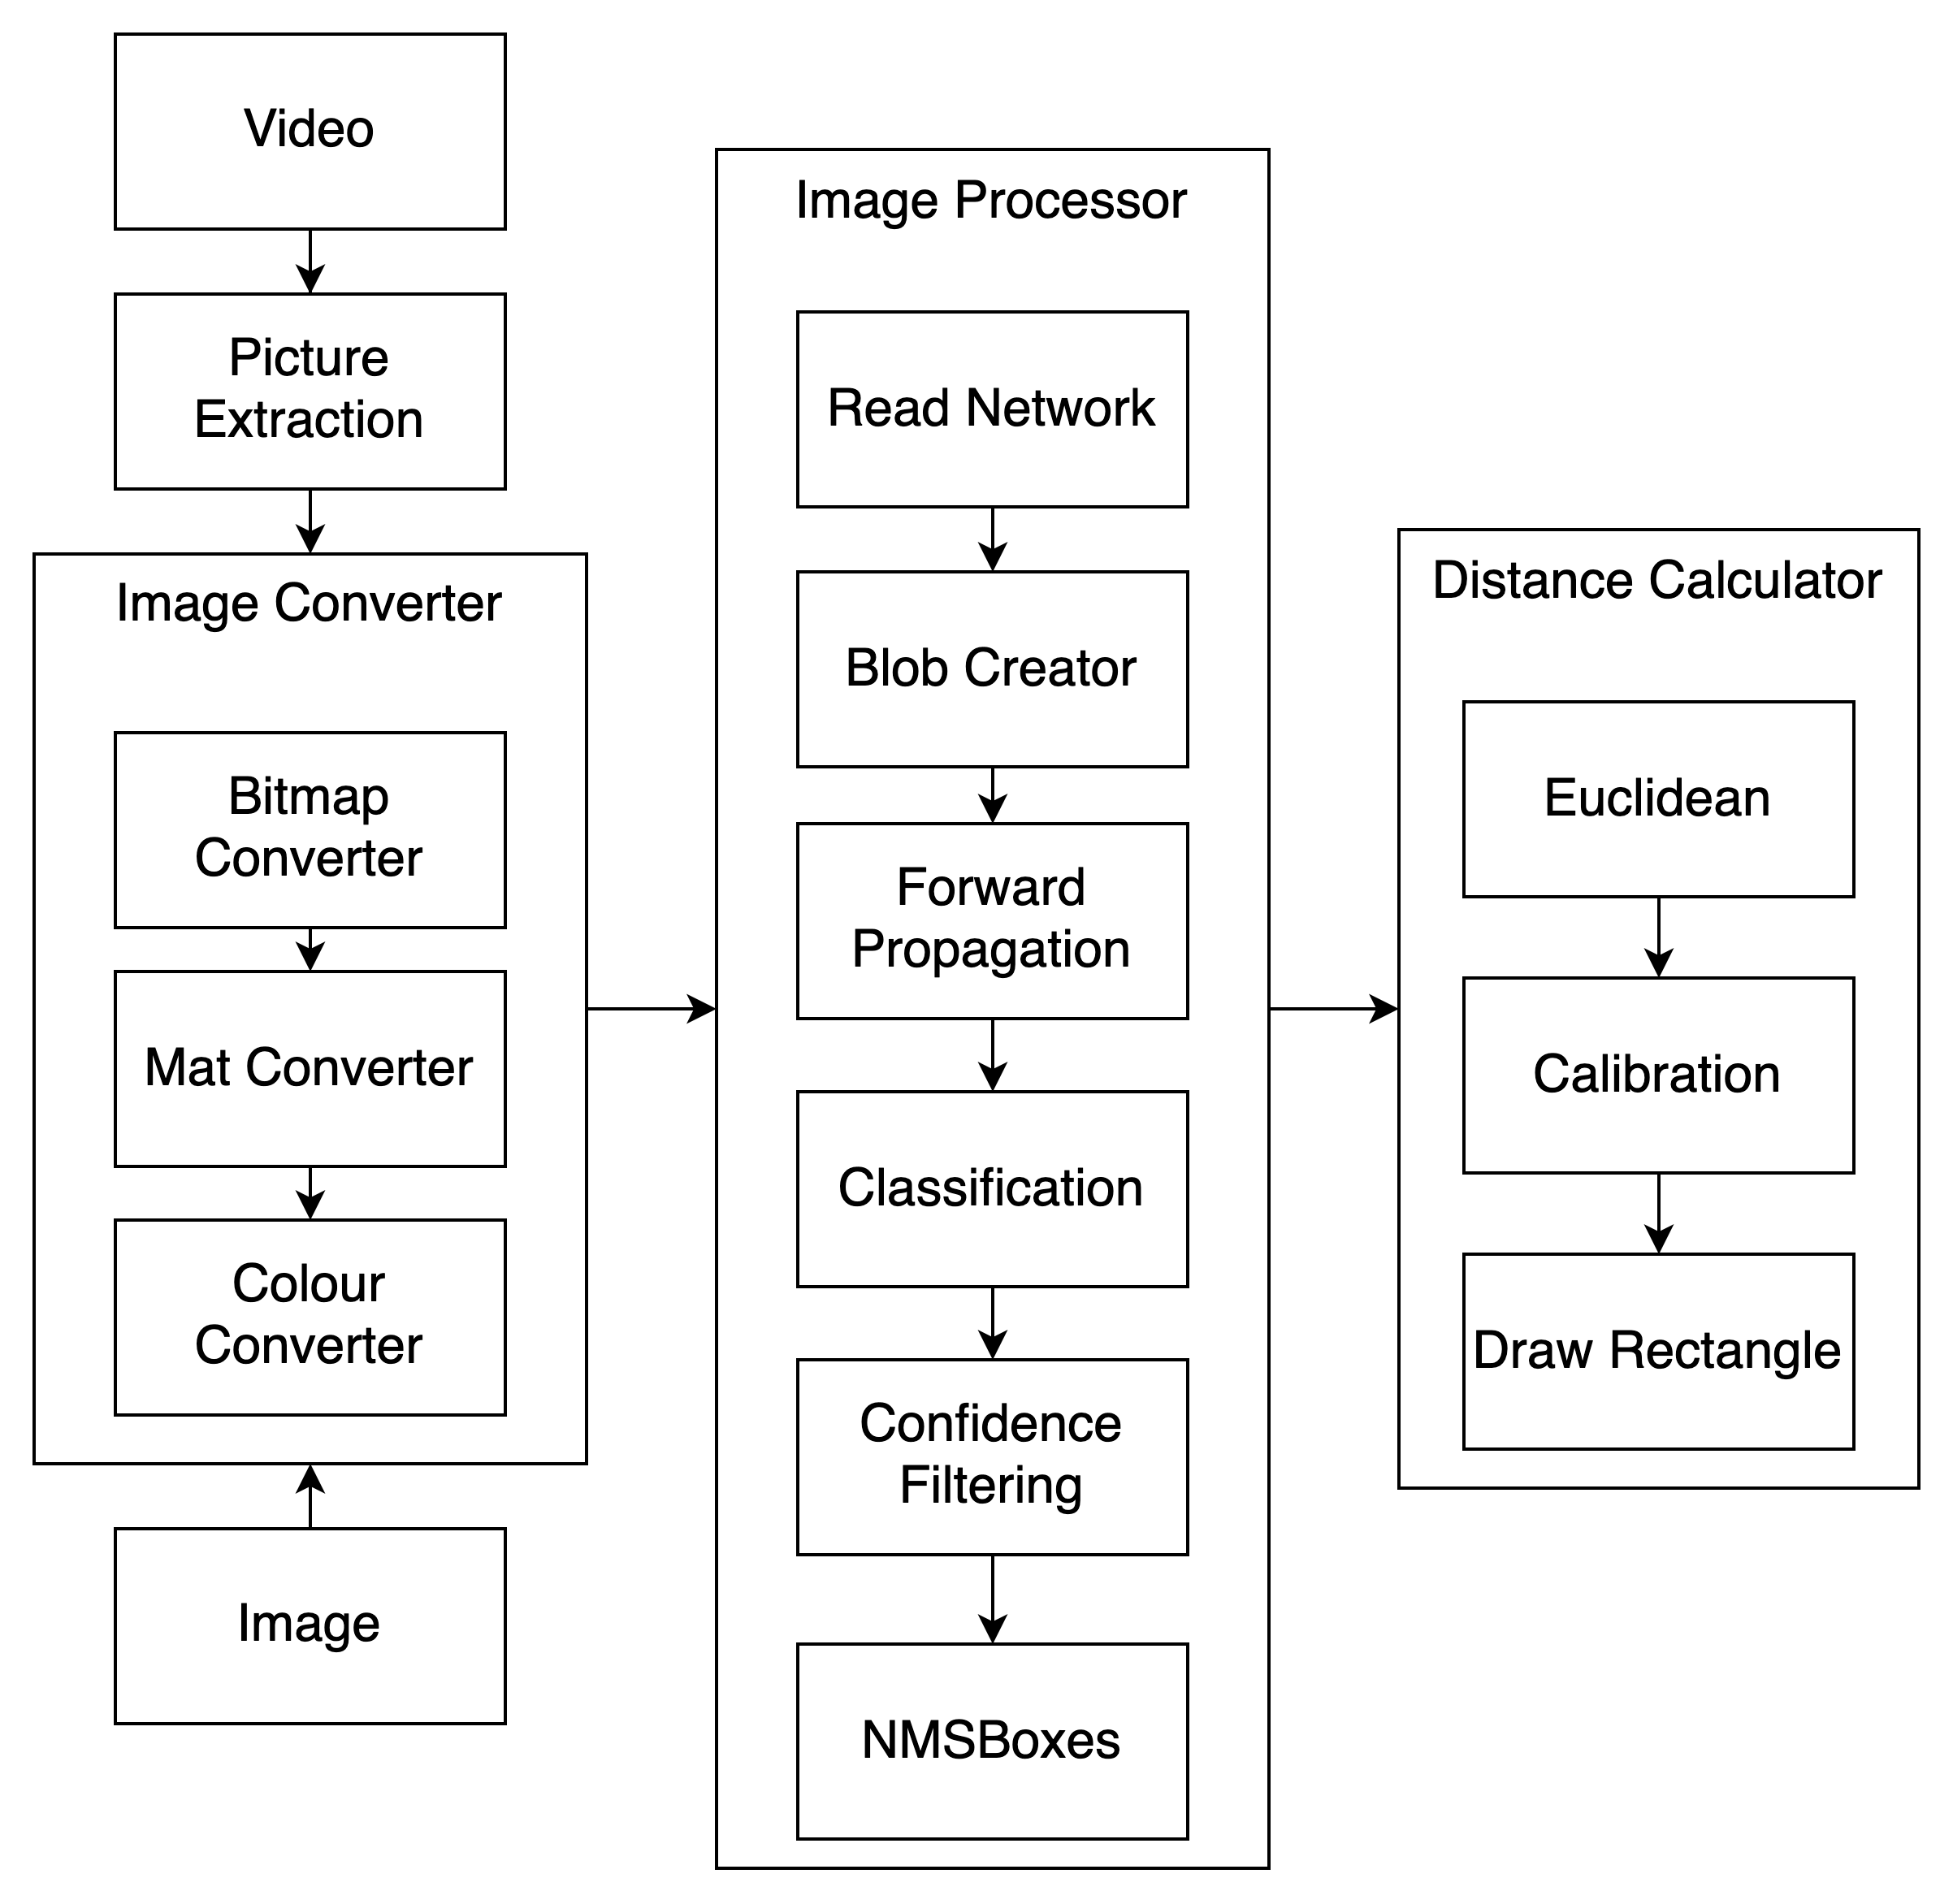
\includegraphics[width=5in]{images/chapter3/system-overview.png}
            \caption{Detection System Overview}
            \label{systemOverview}
        \end{figure}

        The second process is object detection.
        Detection models are set up and configured differently before processing images.
        First of all, YOLO is used with Darknet, which is an open-source neural network framework,
            while MobileNet SSD. MobileNet is used with Caffe framework.
        Then, the threshold will be set for determining the confidence score of the detected object.
            The confidence score threshold of YOLO model will be set to 0.5 or 50 per cent.
            In other words, the detected object will be rejected if YOLO model cannot guarantee that a detected object is human,
            and its confidence score is lower than 50 per cent.
            In contrast, the confidence score threshold of MobileNet SSD model will be set to 0.3 or 30 per cent.
            Because of MobileNet SSD model has a lower ability to detect an object, the confidence threshold is set to be lower.
        After models are set up and configured, the image will be processed in 5 steps.
        For the first step, the pre-processed image will be converted to input blob bypassing Mat image to $blobFromImage()$ function with scale factor.
            Blob will be used for the forward propagation in the neural network.
        Secondly, the blob will be passed to the network through $forward()$ function,
            and the network's output is a list of detected boxes with a label and a confidence score.
        Then, detected objects will be classified.
            Non-human objects will be removed by considering the label of the detected object.
        After that, a confidence score will be filtered by considering the threshold that is set in the configuration step.
        Finally, $NMSBoxes()$ performs non-maximum suppression, which will reduce overlapping detected boxes.

        The last process is determining social distancing.
        After a list of detected object boxes is filtered,
        the distance between each box will be calculated by using the formula which is based on Euclidean distance
        \footnote{an explanation was given in chapter \ref{background}}.
        If the value of the calculated distance is lower than the threshold,
        this means that the couple is too close, and they are breaking social distancing rule.
        The application will change the box's colour to red.
        In contrast, if the value of the calculation is greater than the threshold,
        there is no breaching of social distancing rule, and the box's colour will be changed to green.

    \section{Parallelisation}
        Multithreading is used to reduce the processing time, which can achieve nearly real-time processing.
        The strategy of multithreading is dividing an input video into frames,
        and assign frames to threads by considering a number of available cores.

         There are two things that will be considered while the application is performing multithreading to avoid overheads.
        Firstly, Input/Output (I/O) operation must be avoided by threading.
        Secondly, all variables should be considered due to limited memory.
            For variables, that consume a large space of heap, will be initiated as static by using static block.
            In addition, the usage of the short-lived variable will be reduced to avoid garbage collecting.
            Furthermore, a task will be recycled after thread finished processing the given frame.

        \begin{figure}[!ht]
            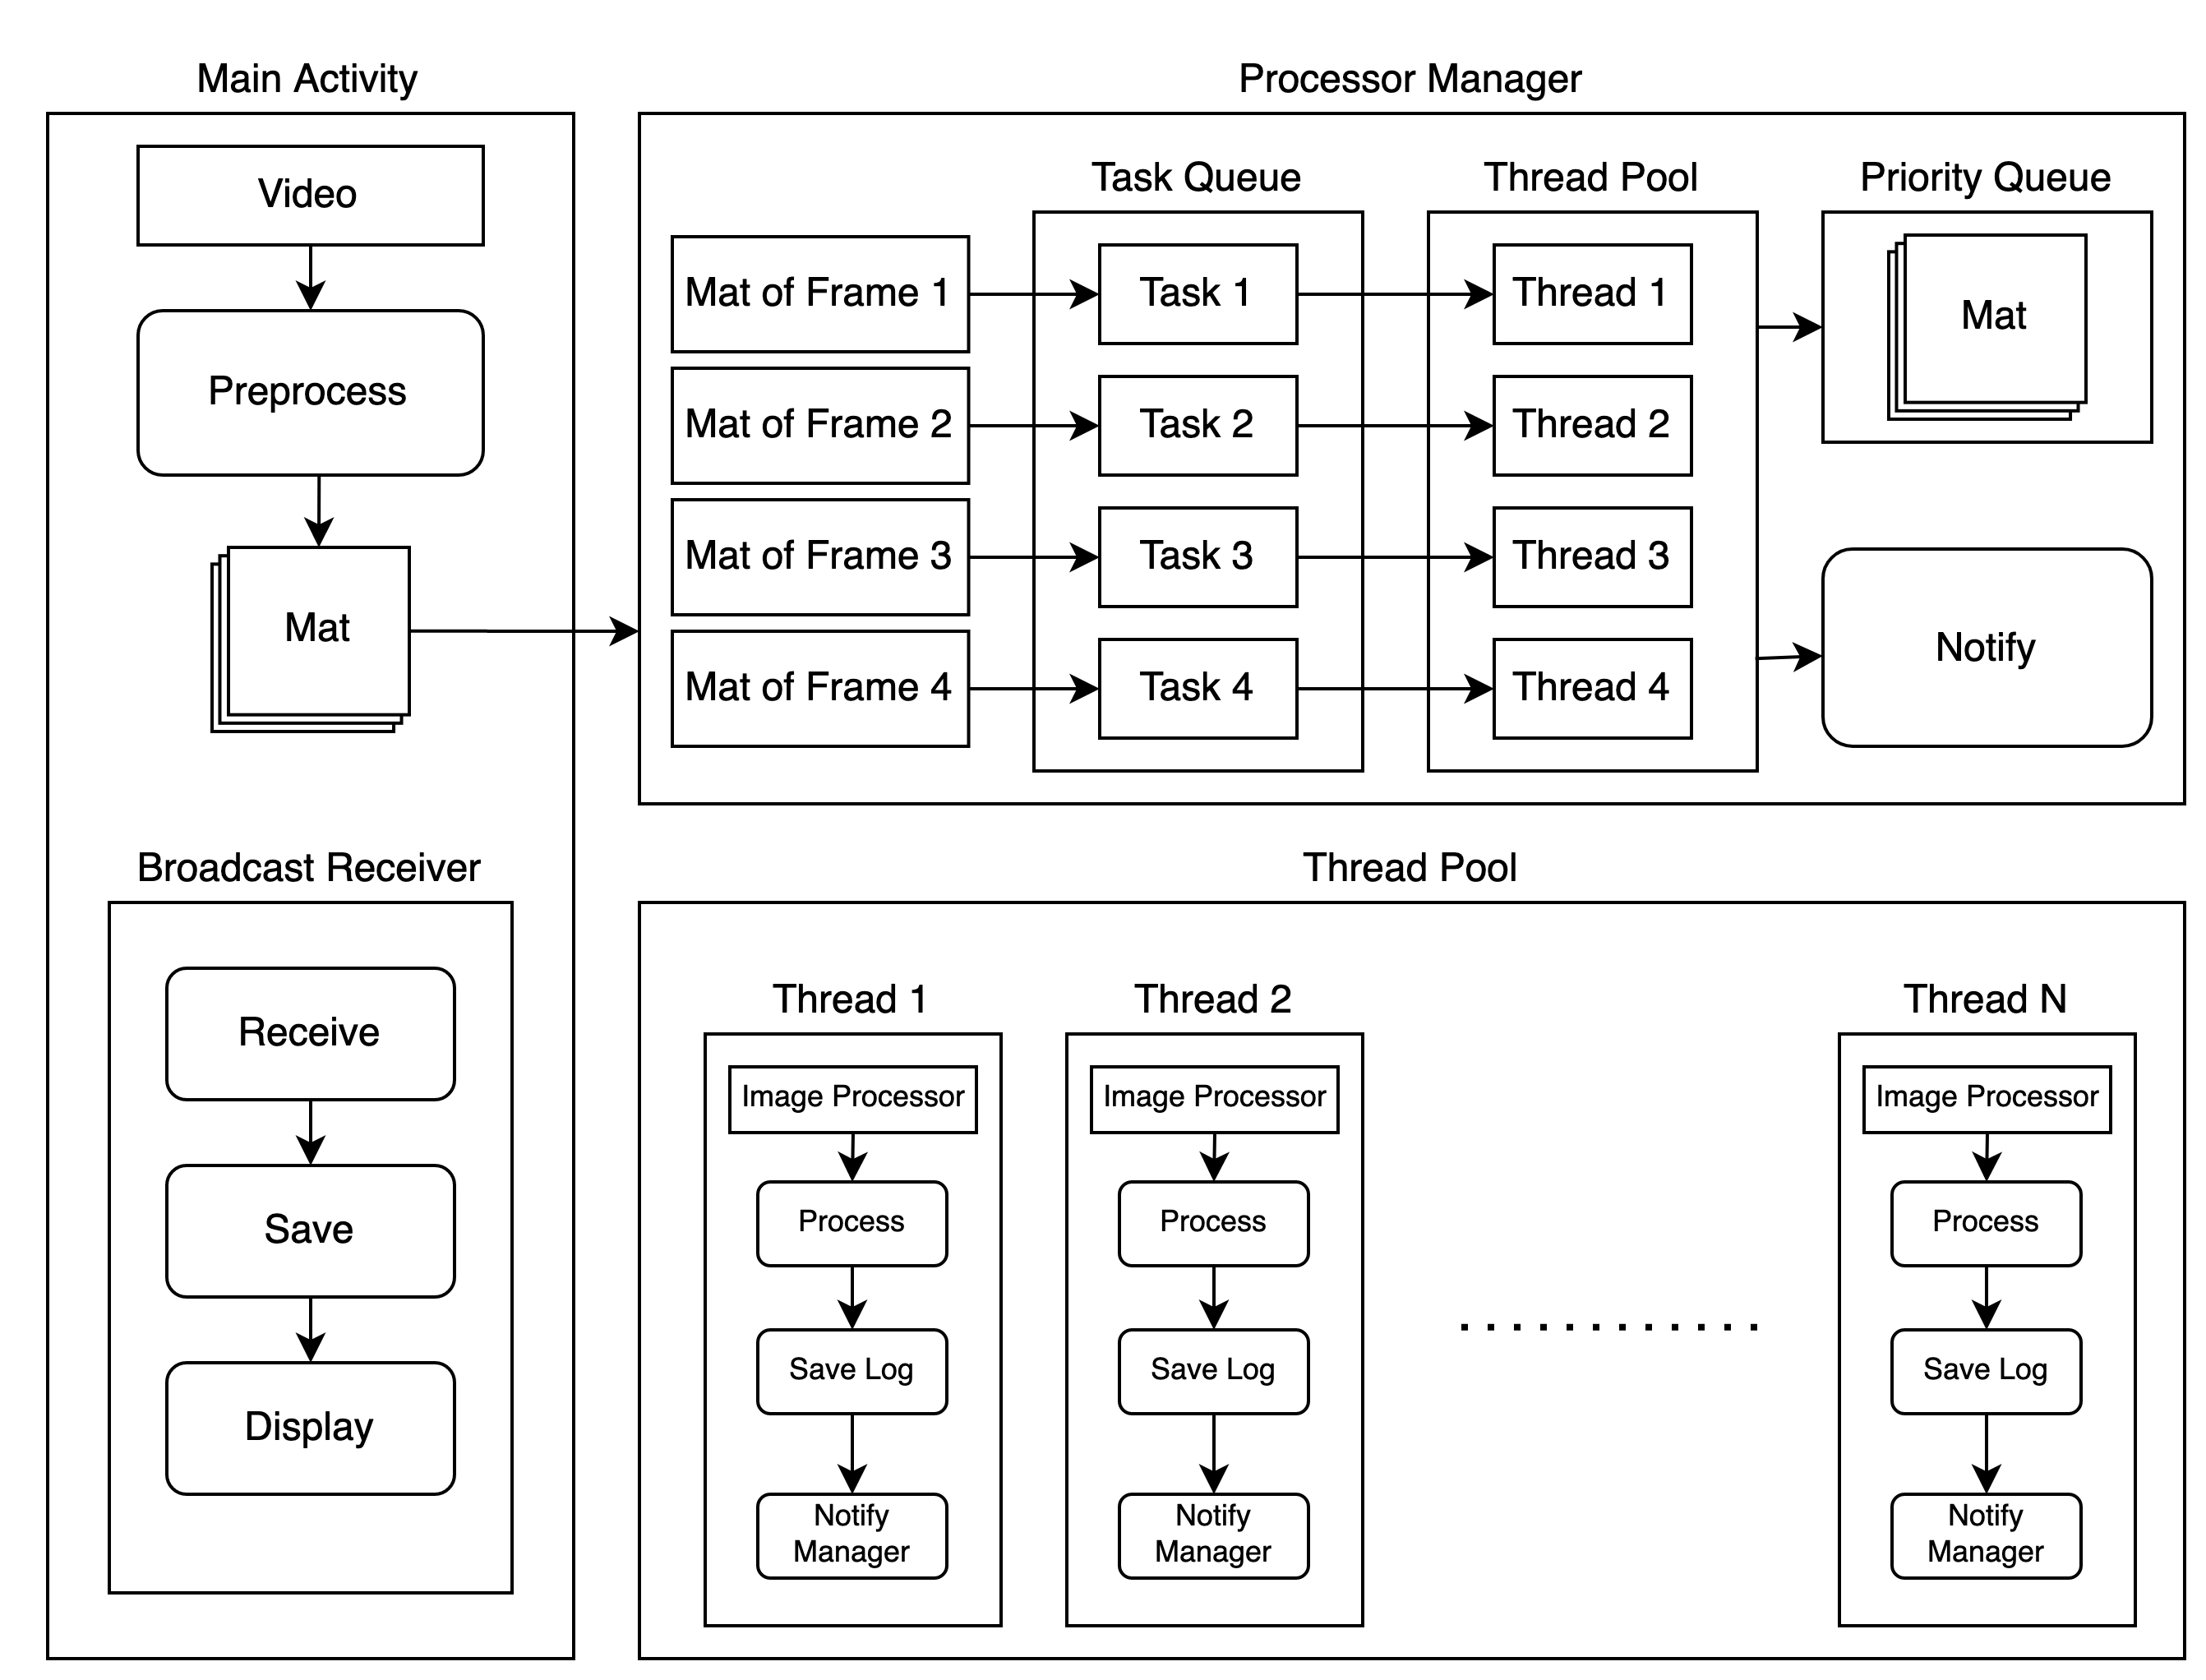
\includegraphics[width=6in]{images/chapter3/parallel.png}
            \caption{Parallel Computing Diagram}
            \label{parallelJava}
        \end{figure}

        To begin with, multithreading in Java, a processor manager is implemented for managing threads efficiently.
        To ensure that the processor manager will be created at once,
        the processor manager is designed with singleton pattern and static block.
        Thread pool and queues are fundamental operators in the processor manager.
        As can be seen in figure \ref{parallelJava}, frames in Mat format will be assigned as a task and queued in TaskQueue.
        Then, tasks will be mapped with thread orderly by the thread pool.
        A working thread will process the given task.
        After a thread finished the given task,
        the thread will write a log regarding social distancing detection, and notify the processor manager.
        Then, a task will be recycled to free up memory.
        When the processor manager receives a notification from workers,
        a processed frame will be retrieved and ordered in the priority queue.
        After the process manager retrieved all processed frames,
        the process manager will notify the main activity.
        All of these processes are run in the background to avoid a frozen application.

        On the other hand, multithreading in C++ is slightly different.
        The central concept of multithreading is the same as Java, except thread management.
        Thread pool is implemented in Java to manage and handle threads,
        while parallelism framework in OpenCV is used in C++.
        This framework is compiled with Threading Building Blocks (TBB), which is developed by Intel.

        \begin{figure}[!ht]
            \centering
            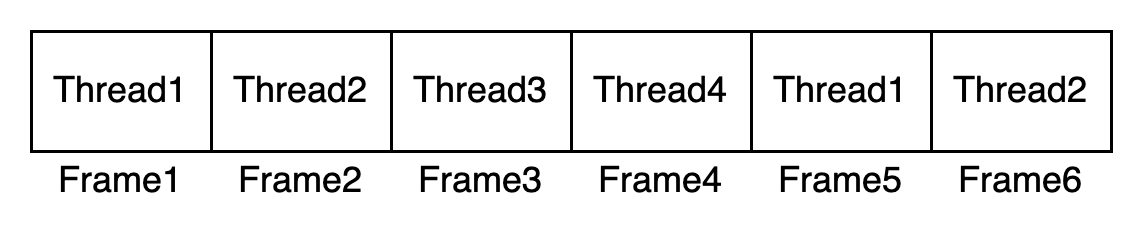
\includegraphics[width=5in]{images/chapter3/cpp-parallel.png}
            \caption{Multithreading in C++}
            \label{parallelCpp}
        \end{figure}

\begin{lstlisting}
    virtual void operator()(const cv::Range& range) const{
        for (size_t i = range.start; i < size; i += threadNo){
            cv::Mat &frame = *(cv::Mat *) frames[i];
            ImageProcessor::process(frame);
        }
    }
\end{lstlisting}

        To reduce the processing time,
        the threads will process the frame which has the same index as itself,
        and the index will be increased by the number of total available cores.
        For example, as can be seen from figure \ref{parallelCpp},
        the first thread will process the first frame and the fifth frame.
        Theoretically, if the frame rate of the video is 30 FPS and there are four threads,
        the first thread will have 100 milliseconds to finish processing the first frame before moving to the fifth frame.

    \section{Frame Rendering}
        The maximum processing frame rate of this application is 10 FPS, which will be discussed in chapter \ref{testing}
        At this frame rate, video cannot be displayed smoothly in live camera;
        thus, there is an algorithm that helps video can be displayed in a higher frame rate.

        First of all, when a frame is streamed from the camera,
        the frame will be considered to be processed or not be processed.
        Processing will be determined from the capability of the device.
        In other words, the maximum processing frame rate will be used as a threshold.
        If a number of processed frames in 1 second exceeds the threshold,
        the frame will not be sent to the processor manager.
        After that, the main activity will check a processed frame in a priority queue from processer manager.
        If there is a processed frame in the priority queue, the processed frame will be displayed to the screen.
        Otherwise, the main activity will read the last log of the processed frame and retrieve all detection rectangles.
        Then, the main activity will draw those rectangles on the incoming frame and display it on the screen.
